\section{Methodology}
\label{sec:Methodology}

\subsection{Data Collection}
We have collected 8 POEM videos of length around 40-45 mins each. Total 8000 snapshots are extracted from these videos. The snapshots are cropped to 720 x 930 pixels. Out of these 24 snapshots are annotated with the help of SAM (Segment\_anything \cite{sam-model})  model with 4 classes: \textit{Background, Muscle layer, Mucosal layer, and Electrode}. The annotated snapshots are used to train the model.

\begin{figure}[ht]
    \centering
    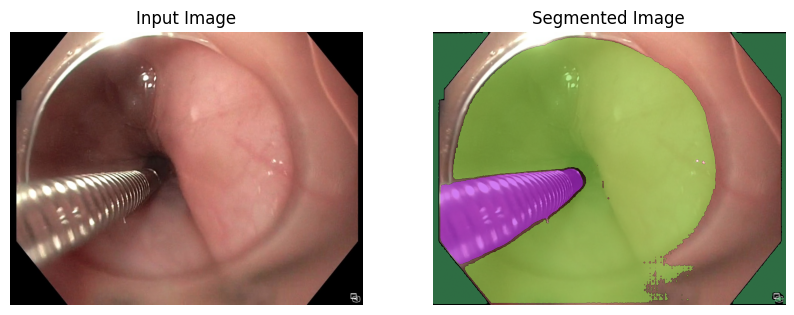
\includegraphics[width=0.4\textwidth]{Images/annoted.png}
    \caption{Annotated image \\ \textit{Background: Green, Muscle layer: Yellow, Electrode: Purple. There is no Mucosal layer in this image.}}
    \label{fig:annotated}
\end{figure}
